\documentclass{whiteboard}
\begin{document}
\begin{frame}[plain,t]
\bbcover{Programação Lógica}{Lógica de Primeira Ordem}{Prof. Edson Alves}{Campus UnB Gama: Faculdade de Ciências e Tecnologias em Engenharia}

\end{frame}
\begin{frame}[plain,t]
\begin{tikzpicture}
\node[draw,opacity=0] at (0, 0) {x};
\node[draw,opacity=0] at (14, 8) {x};

	\node[anchor=west] (title) at (0.0, 7.0) { \Large \bbbold{Variáveis e constantes} };

	\draw[fill=blue!10!white,rounded corners] (0.75, 5.5) rectangle  (13.75, 2.0);

	\draw[color=BBBlue,draw,very thick,rounded corners] (0.75, 5.5) rectangle  (13.75, 2.0);

	\draw[fill=BBBlue,color=BBBlue,draw,very thick,rounded corners] (0.75, 5.5) rectangle  (13.75, 4.5);


	\node[anchor=west,color=white] (a) at (1.0, 5.0) { \bbchalk{Definição} };

	\node[anchor=west,color=white] (b1) at (1.0, 4.0) { \bbtext{Uma \bbbold{variável} é um símbolo que representa um objeto não especificado de um} };

	\node[anchor=west,color=white] (b2) at (1.0, 3.25) { \bbtext{determinado conjunto $U$, o qual é chamado \bbbold{conjunto universal} para a variável.} };

	\node[anchor=west,color=white] (b3) at (1.0, 2.5) { \bbtext{Um membro específico do conjunto universal é denominado \bbbold{constante}.} };


\end{tikzpicture}
\end{frame}
\begin{frame}[plain,t]
\begin{tikzpicture}
\node[draw,opacity=0] at (0, 0) {x};
\node[draw,opacity=0] at (14, 8) {x};

	\node[anchor=west] (title) at (0.0, 7.0) { \Large \bbbold{Termos em Prolog} };

\end{tikzpicture}
\end{frame}
\begin{frame}[plain,t]
\begin{tikzpicture}
\node[draw,opacity=0] at (0, 0) {x};
\node[draw,opacity=0] at (14, 8) {x};

	\node[anchor=west] (title) at (0.0, 7.0) { \Large \bbbold{Termos em Prolog} };


	\node[anchor=west,color=white] (a) at (1.0, 6.0) { $\star$ \bbtext{Prolog tem um único tipo de dado, denominado \bbbold{termo}} };

\end{tikzpicture}
\end{frame}
\begin{frame}[plain,t]
\begin{tikzpicture}
\node[draw,opacity=0] at (0, 0) {x};
\node[draw,opacity=0] at (14, 8) {x};

	\node[anchor=west] (title) at (0.0, 7.0) { \Large \bbbold{Termos em Prolog} };


	\node[anchor=west,color=white] (a) at (1.0, 6.0) { $\star$ \bbtext{Prolog tem um único tipo de dado, denominado \bbbold{termo}} };


	\node[anchor=west,color=white] (b) at (1.0, 5.0) { $\star$ \bbtext{Os argumentos dos predicados Prolog são termos} };

\end{tikzpicture}
\end{frame}
\begin{frame}[plain,t]
\begin{tikzpicture}
\node[draw,opacity=0] at (0, 0) {x};
\node[draw,opacity=0] at (14, 8) {x};

	\node[anchor=west] (title) at (0.0, 7.0) { \Large \bbbold{Termos em Prolog} };


	\node[anchor=west,color=white] (a) at (1.0, 6.0) { $\star$ \bbtext{Prolog tem um único tipo de dado, denominado \bbbold{termo}} };


	\node[anchor=west,color=white] (b) at (1.0, 5.0) { $\star$ \bbtext{Os argumentos dos predicados Prolog são termos} };


	\node[anchor=west,color=white] (c) at (1.0, 4.0) { $\star$ \bbtext{Um \bbbold{átomo} é um nome de propósito geral, composto por uma sequência de} };

	\node[anchor=west,color=white] (c1) at (0.5, 3.5) { \bbtext{caracteres, iniciada com letra minúscula} };

\end{tikzpicture}
\end{frame}
\begin{frame}[plain,t]
\begin{tikzpicture}
\node[draw,opacity=0] at (0, 0) {x};
\node[draw,opacity=0] at (14, 8) {x};

	\node[anchor=west] (title) at (0.0, 7.0) { \Large \bbbold{Termos em Prolog} };


	\node[anchor=west,color=white] (a) at (1.0, 6.0) { $\star$ \bbtext{Prolog tem um único tipo de dado, denominado \bbbold{termo}} };


	\node[anchor=west,color=white] (b) at (1.0, 5.0) { $\star$ \bbtext{Os argumentos dos predicados Prolog são termos} };


	\node[anchor=west,color=white] (c) at (1.0, 4.0) { $\star$ \bbtext{Um \bbbold{átomo} é um nome de propósito geral, composto por uma sequência de} };

	\node[anchor=west,color=white] (c1) at (0.5, 3.5) { \bbtext{caracteres, iniciada com letra minúscula} };

	\node[anchor=west,color=white] (d) at (1.0, 2.5) { $\star$ \bbtext{Delimitar um átomo por aspas simples permite o uso de iniciais maiúsculas e} };

	\node[anchor=west,color=white] (d1) at (0.5, 2.0) { \bbtext{espaços em branco} };

\end{tikzpicture}
\end{frame}
\begin{frame}[plain,t]
\begin{tikzpicture}
\node[draw,opacity=0] at (0, 0) {x};
\node[draw,opacity=0] at (14, 8) {x};

	\node[anchor=west] (title) at (0.0, 7.0) { \Large \bbbold{Termos em Prolog} };


	\node[anchor=west,color=white] (a) at (1.0, 6.0) { $\star$ \bbtext{Prolog tem um único tipo de dado, denominado \bbbold{termo}} };


	\node[anchor=west,color=white] (b) at (1.0, 5.0) { $\star$ \bbtext{Os argumentos dos predicados Prolog são termos} };


	\node[anchor=west,color=white] (c) at (1.0, 4.0) { $\star$ \bbtext{Um \bbbold{átomo} é um nome de propósito geral, composto por uma sequência de} };

	\node[anchor=west,color=white] (c1) at (0.5, 3.5) { \bbtext{caracteres, iniciada com letra minúscula} };

	\node[anchor=west,color=white] (d) at (1.0, 2.5) { $\star$ \bbtext{Delimitar um átomo por aspas simples permite o uso de iniciais maiúsculas e} };

	\node[anchor=west,color=white] (d1) at (0.5, 2.0) { \bbtext{espaços em branco} };

	\node[anchor=west,color=white] (e) at (1.0, 1.0) { $\star$ \bbtext{\bbbold{Números} (inteiros ou flutuantes) são termos primitivos de Prolog} };

\end{tikzpicture}
\end{frame}
\begin{frame}[plain,t]
\vspace*{\fill}

\inputsnippet{prolog}{1}{17}{codes/terms.pl}

\vspace*{\fill}
\end{frame}
\begin{frame}[plain,t]
\begin{tikzpicture}
\node[draw,opacity=0] at (0, 0) {x};
\node[draw,opacity=0] at (14, 8) {x};

	\node[anchor=west] (title) at (0.0, 7.0) { \Large \bbbold{Sentenças abertas} };

	\draw[fill=blue!10!white,rounded corners] (0.25, 5.5) rectangle  (13.75, 1.25);

	\draw[color=BBBlue,draw,very thick,rounded corners] (0.25, 5.5) rectangle  (13.75, 1.25);

	\draw[fill=BBBlue,color=BBBlue,draw,very thick,rounded corners] (0.25, 5.5) rectangle  (13.75, 4.5);

	\node[anchor=west,color=white] (a) at (1.0, 5.0) { \bbchalk{Definição} };

	\node[anchor=west,color=white] (b1) at (0.5, 4.0) { \bbtext{Uma \bbbold{sentença aberta} $S(x)$ em $x$ é uma expressão na qual o símbolo $x$ ocorre} };

	\node[anchor=west,color=white] (b2) at (0.5, 3.25) { \bbtext{uma ou mais vezes e que, caso todas as ocorrências de $x$ sejam substituídas} };

	\node[anchor=west,color=white] (b3) at (0.5, 2.5) { \bbtext{por uma constante $v$ do conjunto universal de $x$, $S(v)$ se torna uma proposição.} };

	\node[anchor=west,color=white] (b4) at (0.5, 1.75) { \bbtext{Sentenças abertas também são chamadas \bbbold{predicados} ou \bbbold{funções proposicionais}.} };

\end{tikzpicture}
\end{frame}
\begin{frame}[plain,t]
\begin{tikzpicture}
\node[draw,opacity=0] at (0, 0) {x};
\node[draw,opacity=0] at (14, 8) {x};

	\node[anchor=west] (title) at (0.0, 7.0) { \Large \bbbold{Variáveis em Prolog} };

\end{tikzpicture}
\end{frame}
\begin{frame}[plain,t]
\begin{tikzpicture}
\node[draw,opacity=0] at (0, 0) {x};
\node[draw,opacity=0] at (14, 8) {x};

	\node[anchor=west] (title) at (0.0, 7.0) { \Large \bbbold{Variáveis em Prolog} };


	\node[anchor=west,color=white] (a) at (1.0, 6.0) { $\star$ \bbtext{Em Prolog, as \bbbold{variáveis} são um subtipo de termo} };

\end{tikzpicture}
\end{frame}
\begin{frame}[plain,t]
\begin{tikzpicture}
\node[draw,opacity=0] at (0, 0) {x};
\node[draw,opacity=0] at (14, 8) {x};

	\node[anchor=west] (title) at (0.0, 7.0) { \Large \bbbold{Variáveis em Prolog} };


	\node[anchor=west,color=white] (a) at (1.0, 6.0) { $\star$ \bbtext{Em Prolog, as \bbbold{variáveis} são um subtipo de termo} };


	\node[anchor=west,color=white] (b) at (1.0, 5.0) { $\star$ \bbtext{Variáveis devem iniciar em letra maiúscula ou com o caractere \code{prolog}{'_'}} };

\end{tikzpicture}
\end{frame}
\begin{frame}[plain,t]
\begin{tikzpicture}
\node[draw,opacity=0] at (0, 0) {x};
\node[draw,opacity=0] at (14, 8) {x};

	\node[anchor=west] (title) at (0.0, 7.0) { \Large \bbbold{Variáveis em Prolog} };


	\node[anchor=west,color=white] (a) at (1.0, 6.0) { $\star$ \bbtext{Em Prolog, as \bbbold{variáveis} são um subtipo de termo} };


	\node[anchor=west,color=white] (b) at (1.0, 5.0) { $\star$ \bbtext{Variáveis devem iniciar em letra maiúscula ou com o caractere \code{prolog}{'_'}} };


	\node[anchor=west,color=white] (c) at (1.0, 4.0) { $\star$ \bbtext{As variáveis permitem a declaração de sentenças abertas em Prolog, denominadas} };

	\node[anchor=west,color=white] (c1) at (0.5, 3.5) { \bbbold{regras} };

\end{tikzpicture}
\end{frame}
\begin{frame}[plain,t]
\begin{tikzpicture}
\node[draw,opacity=0] at (0, 0) {x};
\node[draw,opacity=0] at (14, 8) {x};

	\node[anchor=west] (title) at (0.0, 7.0) { \Large \bbbold{Variáveis em Prolog} };


	\node[anchor=west,color=white] (a) at (1.0, 6.0) { $\star$ \bbtext{Em Prolog, as \bbbold{variáveis} são um subtipo de termo} };


	\node[anchor=west,color=white] (b) at (1.0, 5.0) { $\star$ \bbtext{Variáveis devem iniciar em letra maiúscula ou com o caractere \code{prolog}{'_'}} };


	\node[anchor=west,color=white] (c) at (1.0, 4.0) { $\star$ \bbtext{As variáveis permitem a declaração de sentenças abertas em Prolog, denominadas} };

	\node[anchor=west,color=white] (c1) at (0.5, 3.5) { \bbbold{regras} };

	\node[anchor=west,color=white] (d) at (1.0, 2.5) { $\star$ \bbtext{A sintaxe para a declaração da regra \code{prolog}{rule/N} é} };

	\node[] (d8) at (7.0, 1.0) { \code{prolog}{rule(X1, X2, ..., XN) :- body.} };

\end{tikzpicture}
\end{frame}
\begin{frame}[plain,t]
\begin{tikzpicture}
\node[draw,opacity=0] at (0, 0) {x};
\node[draw,opacity=0] at (14, 8) {x};

	\node[anchor=west] (title) at (0.0, 7.0) { \Large \bbbold{Variáveis em Prolog} };


	\node[anchor=west,color=white] (a) at (1.0, 6.0) { $\star$ \bbtext{Em Prolog, as \bbbold{variáveis} são um subtipo de termo} };


	\node[anchor=west,color=white] (b) at (1.0, 5.0) { $\star$ \bbtext{Variáveis devem iniciar em letra maiúscula ou com o caractere \code{prolog}{'_'}} };


	\node[anchor=west,color=white] (c) at (1.0, 4.0) { $\star$ \bbtext{As variáveis permitem a declaração de sentenças abertas em Prolog, denominadas} };

	\node[anchor=west,color=white] (c1) at (0.5, 3.5) { \bbbold{regras} };

	\node[anchor=west,color=white] (d) at (1.0, 2.5) { $\star$ \bbtext{A sintaxe para a declaração da regra \code{prolog}{rule/N} é} };

	\node[] (d8) at (7.0, 1.0) { \code{prolog}{rule(X1, X2, ..., XN) :- body.} };


	\node[anchor=east] (d1) at (3.5, 1.75) { \bbcomment{nome} };

	\draw[color=BBViolet,thick] (4.0, 1.25) to  (4.8, 1.25);

	\draw[color=BBViolet,-latex,thick] (4.4, 1.25) -- (4.4, 1.75) -- (3.5, 1.75);

\end{tikzpicture}
\end{frame}
\begin{frame}[plain,t]
\begin{tikzpicture}
\node[draw,opacity=0] at (0, 0) {x};
\node[draw,opacity=0] at (14, 8) {x};

	\node[anchor=west] (title) at (0.0, 7.0) { \Large \bbbold{Variáveis em Prolog} };


	\node[anchor=west,color=white] (a) at (1.0, 6.0) { $\star$ \bbtext{Em Prolog, as \bbbold{variáveis} são um subtipo de termo} };


	\node[anchor=west,color=white] (b) at (1.0, 5.0) { $\star$ \bbtext{Variáveis devem iniciar em letra maiúscula ou com o caractere \code{prolog}{'_'}} };


	\node[anchor=west,color=white] (c) at (1.0, 4.0) { $\star$ \bbtext{As variáveis permitem a declaração de sentenças abertas em Prolog, denominadas} };

	\node[anchor=west,color=white] (c1) at (0.5, 3.5) { \bbbold{regras} };

	\node[anchor=west,color=white] (d) at (1.0, 2.5) { $\star$ \bbtext{A sintaxe para a declaração da regra \code{prolog}{rule/N} é} };

	\node[] (d8) at (7.0, 1.0) { \code{prolog}{rule(X1, X2, ..., XN) :- body.} };


	\node[anchor=east] (d1) at (3.5, 1.75) { \bbcomment{nome} };

	\draw[color=BBViolet,thick] (4.0, 1.25) to  (4.8, 1.25);

	\draw[color=BBViolet,-latex,thick] (4.4, 1.25) -- (4.4, 1.75) -- (3.5, 1.75);


	\node[] (d2) at (6.5, -0.1) { \bbcomment{argumentos} };

	\draw[color=BBViolet,thick] (5, 0.8) -- (5, 0.6) -- (8, 0.6) -- (8, 0.8);

	\draw[color=BBViolet,thick,-latex] (6.5, 0.6) to  (6.5, 0.1);


\end{tikzpicture}
\end{frame}
\begin{frame}[plain,t]
\begin{tikzpicture}
\node[draw,opacity=0] at (0, 0) {x};
\node[draw,opacity=0] at (14, 8) {x};

	\node[anchor=west] (title) at (0.0, 7.0) { \Large \bbbold{Variáveis em Prolog} };


	\node[anchor=west,color=white] (a) at (1.0, 6.0) { $\star$ \bbtext{Em Prolog, as \bbbold{variáveis} são um subtipo de termo} };


	\node[anchor=west,color=white] (b) at (1.0, 5.0) { $\star$ \bbtext{Variáveis devem iniciar em letra maiúscula ou com o caractere \code{prolog}{'_'}} };


	\node[anchor=west,color=white] (c) at (1.0, 4.0) { $\star$ \bbtext{As variáveis permitem a declaração de sentenças abertas em Prolog, denominadas} };

	\node[anchor=west,color=white] (c1) at (0.5, 3.5) { \bbbold{regras} };

	\node[anchor=west,color=white] (d) at (1.0, 2.5) { $\star$ \bbtext{A sintaxe para a declaração da regra \code{prolog}{rule/N} é} };

	\node[] (d8) at (7.0, 1.0) { \code{prolog}{rule(X1, X2, ..., XN) :- body.} };


	\node[anchor=east] (d1) at (3.5, 1.75) { \bbcomment{nome} };

	\draw[color=BBViolet,thick] (4.0, 1.25) to  (4.8, 1.25);

	\draw[color=BBViolet,-latex,thick] (4.4, 1.25) -- (4.4, 1.75) -- (3.5, 1.75);


	\node[] (d2) at (6.5, -0.1) { \bbcomment{argumentos} };

	\draw[color=BBViolet,thick] (5, 0.8) -- (5, 0.6) -- (8, 0.6) -- (8, 0.8);

	\draw[color=BBViolet,thick,-latex] (6.5, 0.6) to  (6.5, 0.1);



	\node[anchor=west] (d3) at (8.7, 1.75) { \bbcomment{aridade} };

	\draw[color=BBViolet,thick,-latex] (7.9, 1.2) -- (7.9, 1.75) -- (8.7, 1.75);

\end{tikzpicture}
\end{frame}
\begin{frame}[plain,t]
\begin{tikzpicture}
\node[draw,opacity=0] at (0, 0) {x};
\node[draw,opacity=0] at (14, 8) {x};

	\node[anchor=west] (title) at (0.0, 7.0) { \Large \bbbold{Variáveis em Prolog} };


	\node[anchor=west,color=white] (a) at (1.0, 6.0) { $\star$ \bbtext{Em Prolog, as \bbbold{variáveis} são um subtipo de termo} };


	\node[anchor=west,color=white] (b) at (1.0, 5.0) { $\star$ \bbtext{Variáveis devem iniciar em letra maiúscula ou com o caractere \code{prolog}{'_'}} };


	\node[anchor=west,color=white] (c) at (1.0, 4.0) { $\star$ \bbtext{As variáveis permitem a declaração de sentenças abertas em Prolog, denominadas} };

	\node[anchor=west,color=white] (c1) at (0.5, 3.5) { \bbbold{regras} };

	\node[anchor=west,color=white] (d) at (1.0, 2.5) { $\star$ \bbtext{A sintaxe para a declaração da regra \code{prolog}{rule/N} é} };

	\node[] (d8) at (7.0, 1.0) { \code{prolog}{rule(X1, X2, ..., XN) :- body.} };


	\node[anchor=east] (d1) at (3.5, 1.75) { \bbcomment{nome} };

	\draw[color=BBViolet,thick] (4.0, 1.25) to  (4.8, 1.25);

	\draw[color=BBViolet,-latex,thick] (4.4, 1.25) -- (4.4, 1.75) -- (3.5, 1.75);


	\node[] (d2) at (6.5, -0.1) { \bbcomment{argumentos} };

	\draw[color=BBViolet,thick] (5, 0.8) -- (5, 0.6) -- (8, 0.6) -- (8, 0.8);

	\draw[color=BBViolet,thick,-latex] (6.5, 0.6) to  (6.5, 0.1);



	\node[anchor=west] (d3) at (8.7, 1.75) { \bbcomment{aridade} };

	\draw[color=BBViolet,thick,-latex] (7.9, 1.2) -- (7.9, 1.75) -- (8.7, 1.75);


	\node[anchor=west] (d4) at (10.5, 0.2) { \bbcomment{corpo} };

	\draw[color=BBViolet,thick,-latex] (9.4, 0.8) -- (9.4, 0.2) -- (10.5, 0.2);

\end{tikzpicture}
\end{frame}
\begin{frame}[plain,t]
\begin{tikzpicture}
\node[draw,opacity=0] at (0, 0) {x};
\node[draw,opacity=0] at (14, 8) {x};

	\node[anchor=west] (title) at (0.0, 7.0) { \Large \bbbold{Variáveis em Prolog} };


	\node[anchor=west,color=white] (a) at (1.0, 6.0) { $\star$ \bbtext{Em Prolog, as \bbbold{variáveis} são um subtipo de termo} };


	\node[anchor=west,color=white] (b) at (1.0, 5.0) { $\star$ \bbtext{Variáveis devem iniciar em letra maiúscula ou com o caractere \code{prolog}{'_'}} };


	\node[anchor=west,color=white] (c) at (1.0, 4.0) { $\star$ \bbtext{As variáveis permitem a declaração de sentenças abertas em Prolog, denominadas} };

	\node[anchor=west,color=white] (c1) at (0.5, 3.5) { \bbbold{regras} };

	\node[anchor=west,color=white] (d) at (1.0, 2.5) { $\star$ \bbtext{A sintaxe para a declaração da regra \code{prolog}{rule/N} é} };

	\node[] (d8) at (7.0, 1.0) { \code{prolog}{rule(X1, X2, ..., XN) :- body.} };


	\node[anchor=east] (d1) at (3.5, 1.75) { \bbcomment{nome} };

	\draw[color=BBViolet,thick] (4.0, 1.25) to  (4.8, 1.25);

	\draw[color=BBViolet,-latex,thick] (4.4, 1.25) -- (4.4, 1.75) -- (3.5, 1.75);


	\node[] (d2) at (6.5, -0.1) { \bbcomment{argumentos} };

	\draw[color=BBViolet,thick] (5, 0.8) -- (5, 0.6) -- (8, 0.6) -- (8, 0.8);

	\draw[color=BBViolet,thick,-latex] (6.5, 0.6) to  (6.5, 0.1);



	\node[anchor=west] (d3) at (8.7, 1.75) { \bbcomment{aridade} };

	\draw[color=BBViolet,thick,-latex] (7.9, 1.2) -- (7.9, 1.75) -- (8.7, 1.75);


	\node[anchor=west] (d4) at (10.5, 0.2) { \bbcomment{corpo} };

	\draw[color=BBViolet,thick,-latex] (9.4, 0.8) -- (9.4, 0.2) -- (10.5, 0.2);


	\node[anchor=west] (d5) at (11.5, 0.92) { \bbcomment{terminador} };

	\draw[color=BBViolet,thick,-latex] (10, 0.92) -- (11.5, 0.92);


\end{tikzpicture}
\end{frame}
\begin{frame}[plain,t]
\begin{tikzpicture}
\node[draw,opacity=0] at (0, 0) {x};
\node[draw,opacity=0] at (14, 8) {x};

	\node[anchor=west] (title) at (0.0, 7.0) { \Large \bbbold{Declarando regras em Prolog} };

\end{tikzpicture}
\end{frame}
\begin{frame}[plain,t]
\begin{tikzpicture}
\node[draw,opacity=0] at (0, 0) {x};
\node[draw,opacity=0] at (14, 8) {x};

	\node[anchor=west] (title) at (0.0, 7.0) { \Large \bbbold{Declarando regras em Prolog} };


	\node[anchor=west] (a) at (1.0, 6.0) { $\star$ \bbtext{Assim como os fatos, as regras devem ser declaradas em um arquivo `\bblink{.pl}}' };

\end{tikzpicture}
\end{frame}
\begin{frame}[plain,t]
\begin{tikzpicture}
\node[draw,opacity=0] at (0, 0) {x};
\node[draw,opacity=0] at (14, 8) {x};

	\node[anchor=west] (title) at (0.0, 7.0) { \Large \bbbold{Declarando regras em Prolog} };


	\node[anchor=west] (a) at (1.0, 6.0) { $\star$ \bbtext{Assim como os fatos, as regras devem ser declaradas em um arquivo `\bblink{.pl}}' };


	\node[anchor=west] (b) at (1.0, 5.0) { $\star$ \bbtext{O corpo de uma regra deve ou ser uma proposição composta ou ser omitido} };

\end{tikzpicture}
\end{frame}
\begin{frame}[plain,t]
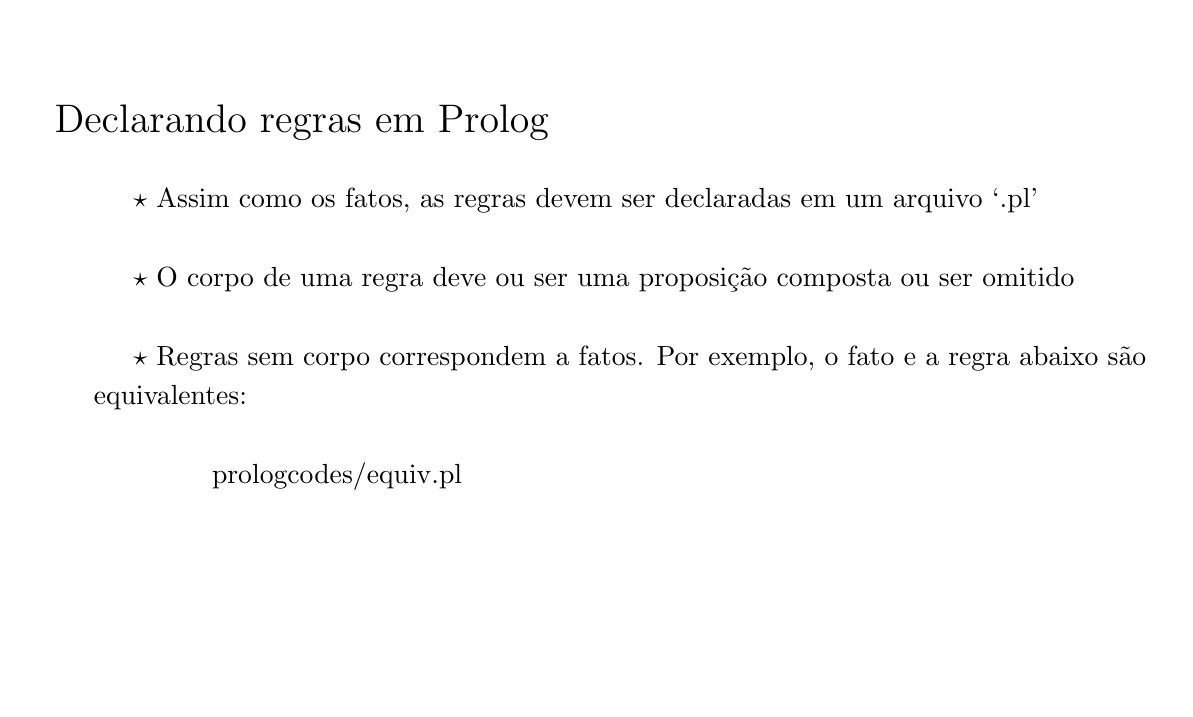
\begin{tikzpicture}
\node[draw,opacity=0] at (0, 0) {x};
\node[draw,opacity=0] at (14, 8) {x};

	\node[anchor=west] (title) at (0.0, 7.0) { \Large \bbbold{Declarando regras em Prolog} };


	\node[anchor=west] (a) at (1.0, 6.0) { $\star$ \bbtext{Assim como os fatos, as regras devem ser declaradas em um arquivo `\bblink{.pl}}' };


	\node[anchor=west] (b) at (1.0, 5.0) { $\star$ \bbtext{O corpo de uma regra deve ou ser uma proposição composta ou ser omitido} };


	\node[anchor=west] (c) at (1.0, 4.0) { $\star$ \bbtext{Regras sem corpo correspondem a fatos. Por exemplo, o fato e a regra abaixo são } };

	\node[anchor=west] (c1) at (0.5, 3.5) { \bbtext{equivalentes:} };

	\node[anchor=west] (c2) at (2.0, 2.5) { \inputsyntax{prolog}{codes/equiv.pl} };

\end{tikzpicture}
\end{frame}
\begin{frame}[plain,t]
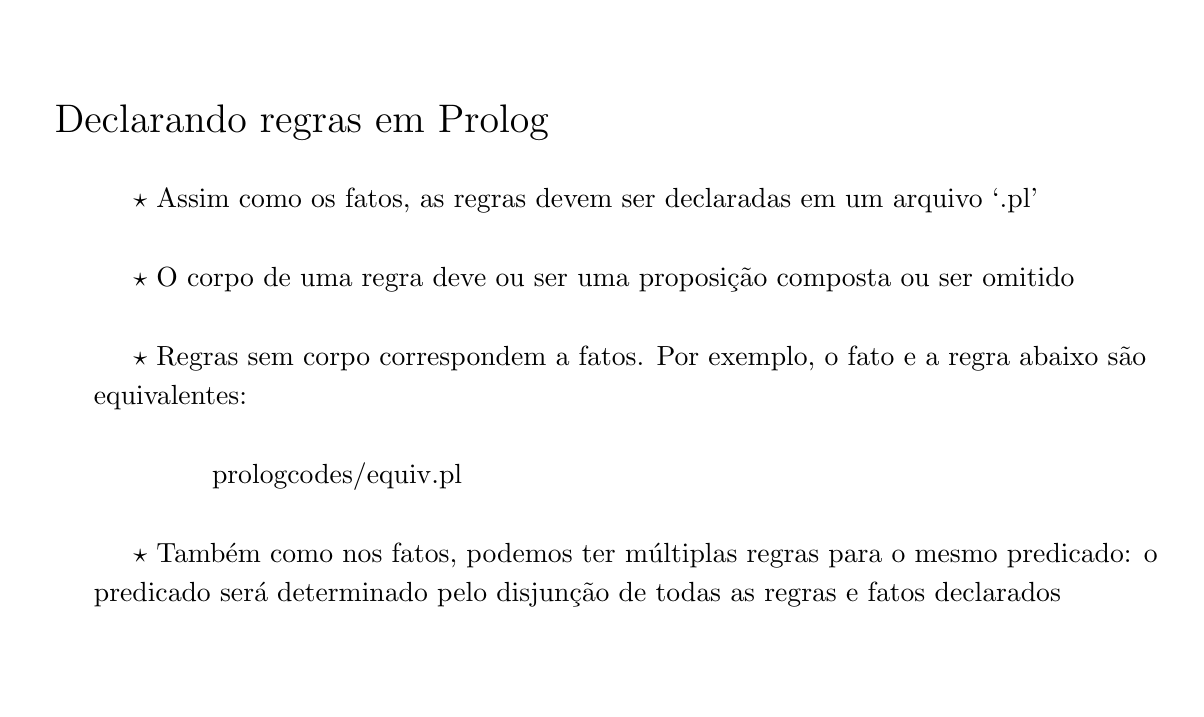
\begin{tikzpicture}
\node[draw,opacity=0] at (0, 0) {x};
\node[draw,opacity=0] at (14, 8) {x};

	\node[anchor=west] (title) at (0.0, 7.0) { \Large \bbbold{Declarando regras em Prolog} };


	\node[anchor=west] (a) at (1.0, 6.0) { $\star$ \bbtext{Assim como os fatos, as regras devem ser declaradas em um arquivo `\bblink{.pl}}' };


	\node[anchor=west] (b) at (1.0, 5.0) { $\star$ \bbtext{O corpo de uma regra deve ou ser uma proposição composta ou ser omitido} };


	\node[anchor=west] (c) at (1.0, 4.0) { $\star$ \bbtext{Regras sem corpo correspondem a fatos. Por exemplo, o fato e a regra abaixo são } };

	\node[anchor=west] (c1) at (0.5, 3.5) { \bbtext{equivalentes:} };

	\node[anchor=west] (c2) at (2.0, 2.5) { \inputsyntax{prolog}{codes/equiv.pl} };


	\node[anchor=west] (d) at (1.0, 1.5) { $\star$ \bbtext{Também como nos fatos, podemos ter múltiplas regras para o mesmo predicado: o } };

	\node[anchor=west] (d1) at (0.5, 1.0) { \bbtext{predicado será determinado pelo disjunção de todas as regras e fatos declarados} };

\end{tikzpicture}
\end{frame}
\begin{frame}[plain,t]
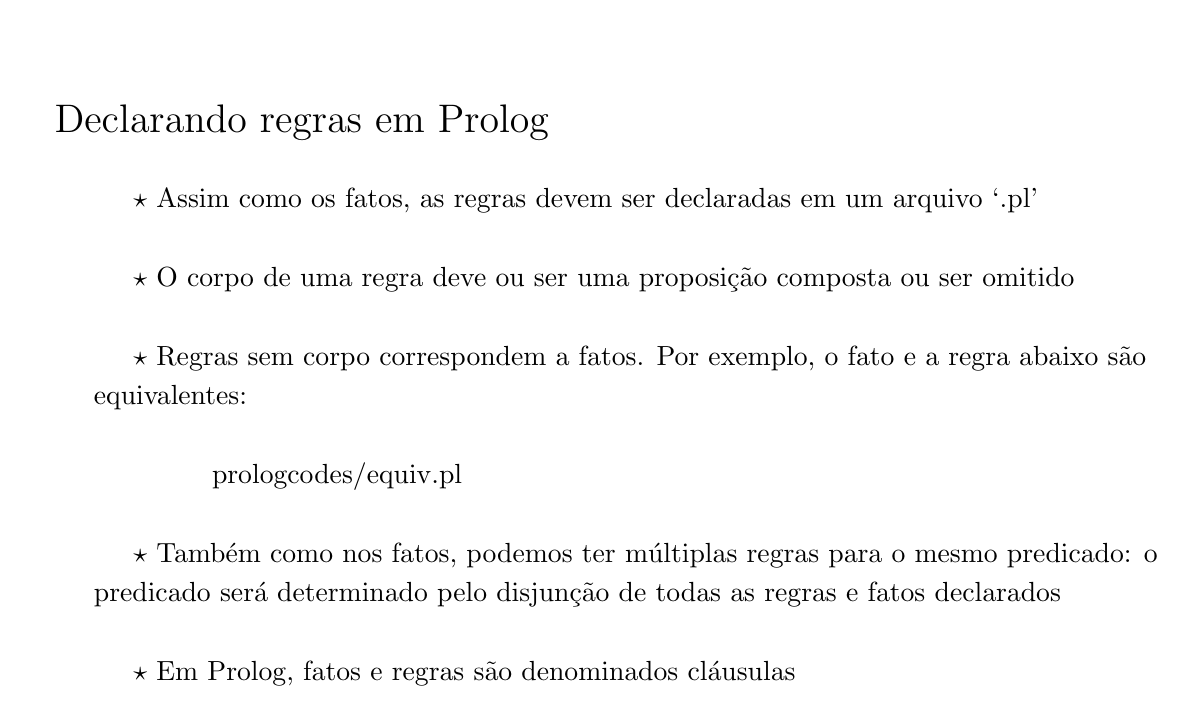
\begin{tikzpicture}
\node[draw,opacity=0] at (0, 0) {x};
\node[draw,opacity=0] at (14, 8) {x};

	\node[anchor=west] (title) at (0.0, 7.0) { \Large \bbbold{Declarando regras em Prolog} };


	\node[anchor=west] (a) at (1.0, 6.0) { $\star$ \bbtext{Assim como os fatos, as regras devem ser declaradas em um arquivo `\bblink{.pl}}' };


	\node[anchor=west] (b) at (1.0, 5.0) { $\star$ \bbtext{O corpo de uma regra deve ou ser uma proposição composta ou ser omitido} };


	\node[anchor=west] (c) at (1.0, 4.0) { $\star$ \bbtext{Regras sem corpo correspondem a fatos. Por exemplo, o fato e a regra abaixo são } };

	\node[anchor=west] (c1) at (0.5, 3.5) { \bbtext{equivalentes:} };

	\node[anchor=west] (c2) at (2.0, 2.5) { \inputsyntax{prolog}{codes/equiv.pl} };


	\node[anchor=west] (d) at (1.0, 1.5) { $\star$ \bbtext{Também como nos fatos, podemos ter múltiplas regras para o mesmo predicado: o } };

	\node[anchor=west] (d1) at (0.5, 1.0) { \bbtext{predicado será determinado pelo disjunção de todas as regras e fatos declarados} };


	\node[anchor=west] (e) at (1.0, 0.0) { $\star$ \bbtext{Em Prolog, fatos e regras são denominados \bbbold{cláusulas}} };

\end{tikzpicture}
\end{frame}
\begin{frame}[plain,t]
\vspace*{\fill}

\inputsnippet{prolog}{1}{18}{codes/rules.pl}

\vspace*{\fill}
\end{frame}
\begin{frame}[plain,t]
\begin{tikzpicture}
\node[draw,opacity=0] at (0, 0) {x};
\node[draw,opacity=0] at (14, 8) {x};

	\node[anchor=west] (title) at (0.0, 7.0) { \Large \bbbold{Quantificador existencial} };

	\draw[fill=blue!10!white,rounded corners] (0.75, 5.5) rectangle  (13.5, 2.0);

	\draw[color=BBBlue,draw,very thick,rounded corners] (0.75, 5.5) rectangle  (13.5, 2.0);

	\draw[fill=BBBlue,color=BBBlue,draw,very thick,rounded corners] (0.75, 5.5) rectangle  (13.5, 4.5);


	\node[anchor=west,color=white] (a) at (1.0, 5.0) { \bbchalk{Definição} };

	\node[anchor=west,color=white] (b1) at (1.0, 4.0) { \bbtext{Sejam $S(x)$ uma sentença aberta. O quantificador \bbbold{existencial} $\exists$ é utilizado} };

	\node[anchor=west,color=white] (b2) at (1.0, 3.25) { \bbtext{na construção $\exists x.S(x)$, a qual significa que existe pelo menos um elemento } };

	\node[anchor=west,color=white] (b3) at (1.0, 2.5) { \bbtext{$v$ no conjunto universal de $x$ tal que $S(v)$ é verdadeira.} };

\end{tikzpicture}
\end{frame}
\begin{frame}[plain,t]
\begin{tikzpicture}
\node[draw,opacity=0] at (0, 0) {x};
\node[draw,opacity=0] at (14, 8) {x};

	\node[anchor=west] (title) at (0.0, 7.0) { \Large \bbbold{Consultas simples} };

\end{tikzpicture}
\end{frame}
\begin{frame}[plain,t]
\begin{tikzpicture}
\node[draw,opacity=0] at (0, 0) {x};
\node[draw,opacity=0] at (14, 8) {x};

	\node[anchor=west] (title) at (0.0, 7.0) { \Large \bbbold{Consultas simples} };

	\node[anchor=west] (a) at (1.0, 6.0) { $\star$ \bbtext{Em Prolog, quantificador existencial está associado às consultas} };

\end{tikzpicture}
\end{frame}
\begin{frame}[plain,t]
\begin{tikzpicture}
\node[draw,opacity=0] at (0, 0) {x};
\node[draw,opacity=0] at (14, 8) {x};

	\node[anchor=west] (title) at (0.0, 7.0) { \Large \bbbold{Consultas simples} };

	\node[anchor=west] (a) at (1.0, 6.0) { $\star$ \bbtext{Em Prolog, quantificador existencial está associado às consultas} };

	\node[anchor=west] (b) at (1.0, 5.0) { $\star$ \bbtext{Uma \bbbold{consulta simples} corresponde a uma sentença aberta simples, isto é, um } };

	\node[anchor=west] (b1) at (0.5, 4.5) { \bbtext{predicado e seus respectivos argumentos} };

\end{tikzpicture}
\end{frame}
\begin{frame}[plain,t]
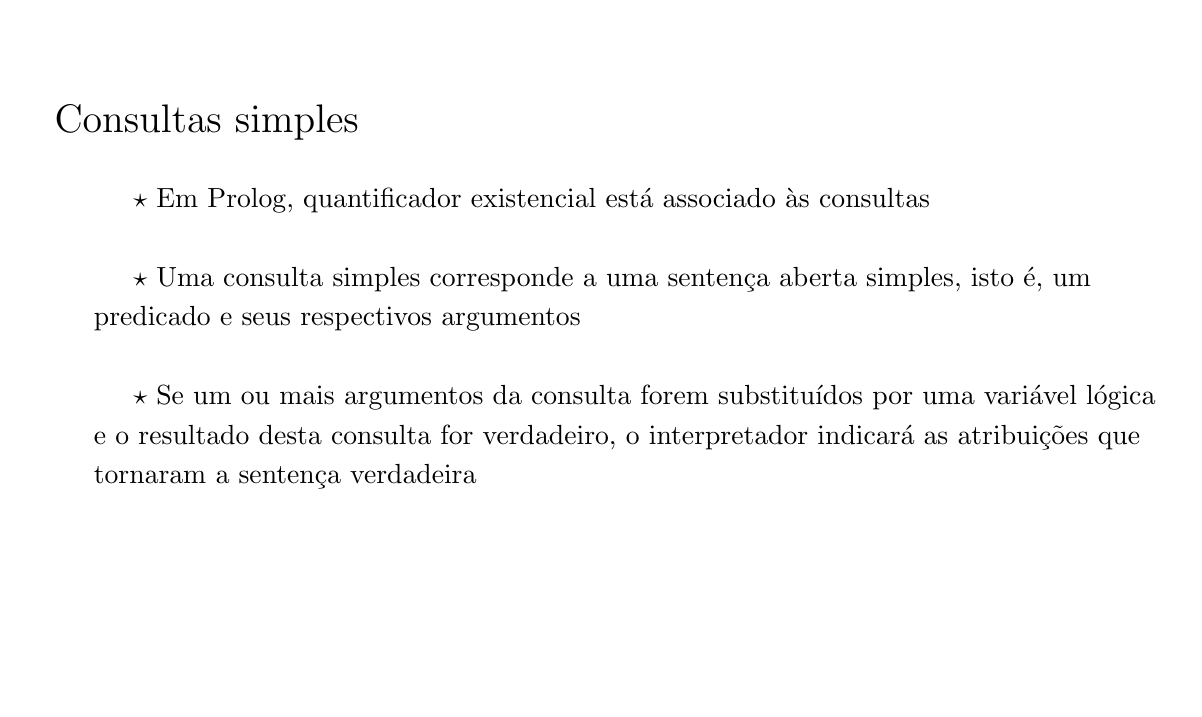
\begin{tikzpicture}
\node[draw,opacity=0] at (0, 0) {x};
\node[draw,opacity=0] at (14, 8) {x};

	\node[anchor=west] (title) at (0.0, 7.0) { \Large \bbbold{Consultas simples} };

	\node[anchor=west] (a) at (1.0, 6.0) { $\star$ \bbtext{Em Prolog, quantificador existencial está associado às consultas} };

	\node[anchor=west] (b) at (1.0, 5.0) { $\star$ \bbtext{Uma \bbbold{consulta simples} corresponde a uma sentença aberta simples, isto é, um } };

	\node[anchor=west] (b1) at (0.5, 4.5) { \bbtext{predicado e seus respectivos argumentos} };

	\node[anchor=west] (c) at (1.0, 3.5) { $\star$ \bbtext{Se um ou mais argumentos da consulta forem substituídos por uma variável lógica } };

	\node[anchor=west] (c1) at (0.5, 3.0) { \bbtext{e o resultado desta consulta for verdadeiro, o interpretador indicará as atribuições que} };

	\node[anchor=west] (c2) at (0.5, 2.5) { \bbtext{tornaram a sentença verdadeira} };

\end{tikzpicture}
\end{frame}
\begin{frame}[plain,t]
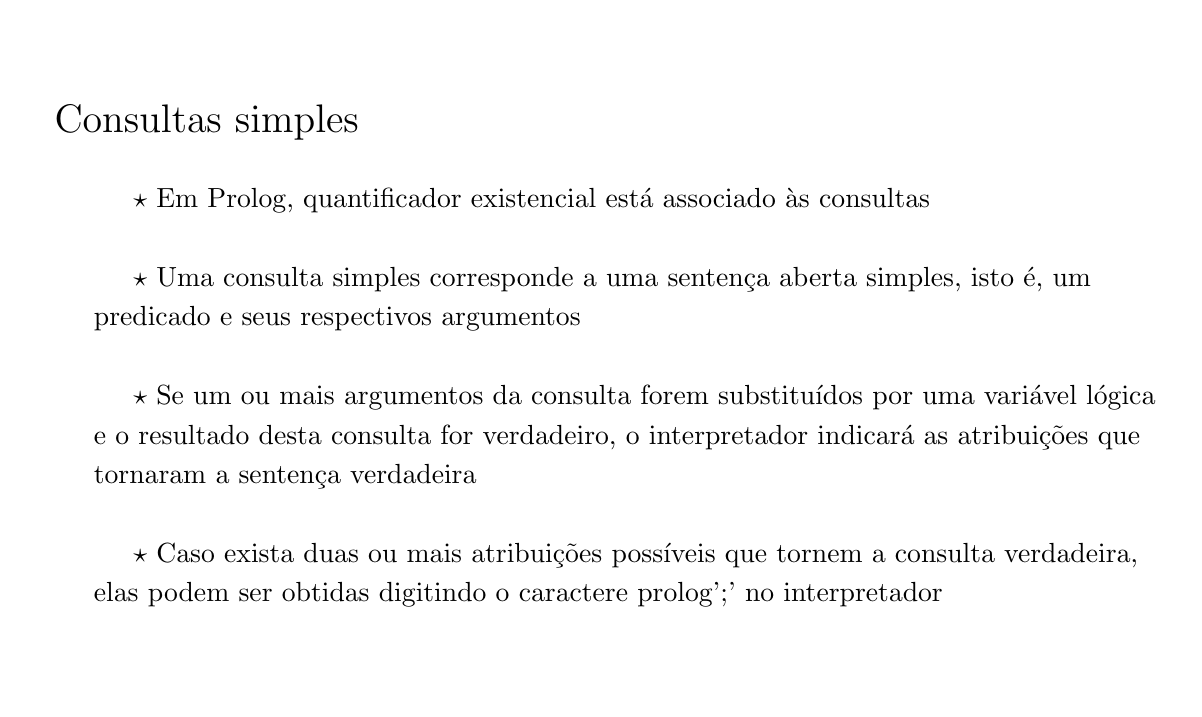
\begin{tikzpicture}
\node[draw,opacity=0] at (0, 0) {x};
\node[draw,opacity=0] at (14, 8) {x};

	\node[anchor=west] (title) at (0.0, 7.0) { \Large \bbbold{Consultas simples} };

	\node[anchor=west] (a) at (1.0, 6.0) { $\star$ \bbtext{Em Prolog, quantificador existencial está associado às consultas} };

	\node[anchor=west] (b) at (1.0, 5.0) { $\star$ \bbtext{Uma \bbbold{consulta simples} corresponde a uma sentença aberta simples, isto é, um } };

	\node[anchor=west] (b1) at (0.5, 4.5) { \bbtext{predicado e seus respectivos argumentos} };

	\node[anchor=west] (c) at (1.0, 3.5) { $\star$ \bbtext{Se um ou mais argumentos da consulta forem substituídos por uma variável lógica } };

	\node[anchor=west] (c1) at (0.5, 3.0) { \bbtext{e o resultado desta consulta for verdadeiro, o interpretador indicará as atribuições que} };

	\node[anchor=west] (c2) at (0.5, 2.5) { \bbtext{tornaram a sentença verdadeira} };

	\node[anchor=west] (d) at (1.0, 1.5) { $\star$ \bbtext{Caso exista duas ou mais atribuições possíveis que tornem a consulta verdadeira,} };

	\node[anchor=west] (d1) at (0.5, 1.0) { \bbtext{elas podem ser obtidas digitindo o caractere \code{prolog}{';'} no interpretador} };

\end{tikzpicture}
\end{frame}
\begin{frame}[plain,t]
\vspace*{\fill}

\inputsnippet{prolog}{1}{18}{codes/consult.pl}

\vspace*{\fill}
\end{frame}
\begin{frame}[plain,t]
\begin{tikzpicture}
\node[draw,opacity=0] at (0, 0) {x};
\node[draw,opacity=0] at (14, 8) {x};

	\node[anchor=west] (title) at (0.0, 7.0) { \Large \bbbold{Consultas e variáveis lógicas} };

\end{tikzpicture}
\end{frame}
\begin{frame}[plain,t]
\begin{tikzpicture}
\node[draw,opacity=0] at (0, 0) {x};
\node[draw,opacity=0] at (14, 8) {x};

	\node[anchor=west] (title) at (0.0, 7.0) { \Large \bbbold{Consultas e variáveis lógicas} };


	\node[anchor=west] (a) at (1.0, 6.0) { $\star$ \bbtext{As consultas em Prolog são avaliadas por meio de um mecanismo de casamento de} };

	\node[anchor=west] (a1) at (0.5, 5.5) { \bbtext{padrões denominado \bbbold{unificação}} };

\end{tikzpicture}
\end{frame}
\begin{frame}[plain,t]
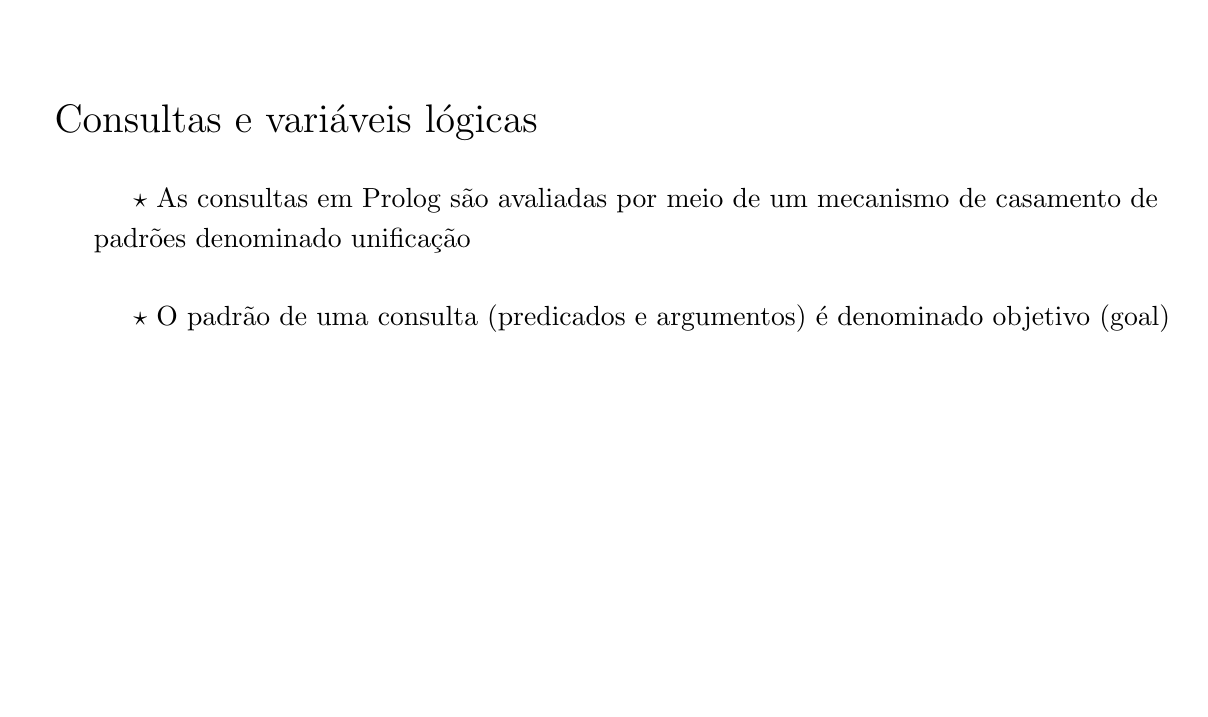
\begin{tikzpicture}
\node[draw,opacity=0] at (0, 0) {x};
\node[draw,opacity=0] at (14, 8) {x};

	\node[anchor=west] (title) at (0.0, 7.0) { \Large \bbbold{Consultas e variáveis lógicas} };


	\node[anchor=west] (a) at (1.0, 6.0) { $\star$ \bbtext{As consultas em Prolog são avaliadas por meio de um mecanismo de casamento de} };

	\node[anchor=west] (a1) at (0.5, 5.5) { \bbtext{padrões denominado \bbbold{unificação}} };


	\node[anchor=west] (b) at (1.0, 4.5) { $\star$ \bbtext{O padrão de uma consulta (predicados e argumentos) é denominado \bbbold{objetivo} (\bbenglish{goal})} };

\end{tikzpicture}
\end{frame}
\begin{frame}[plain,t]
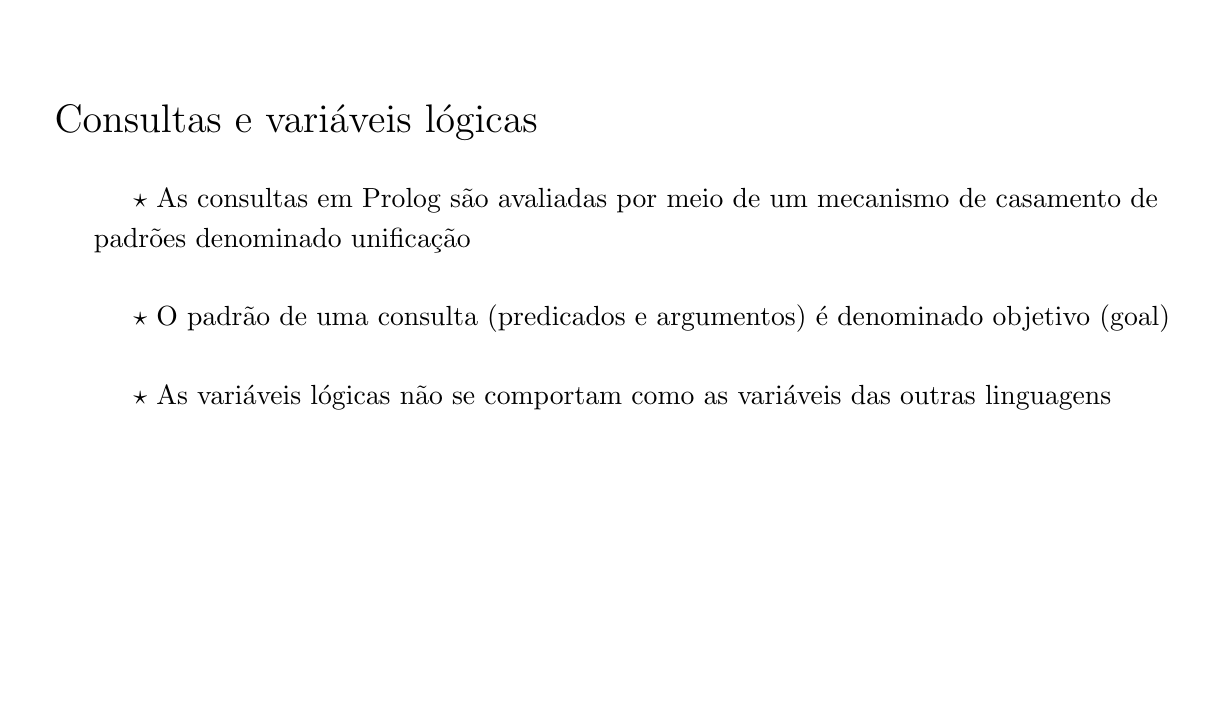
\begin{tikzpicture}
\node[draw,opacity=0] at (0, 0) {x};
\node[draw,opacity=0] at (14, 8) {x};

	\node[anchor=west] (title) at (0.0, 7.0) { \Large \bbbold{Consultas e variáveis lógicas} };


	\node[anchor=west] (a) at (1.0, 6.0) { $\star$ \bbtext{As consultas em Prolog são avaliadas por meio de um mecanismo de casamento de} };

	\node[anchor=west] (a1) at (0.5, 5.5) { \bbtext{padrões denominado \bbbold{unificação}} };


	\node[anchor=west] (b) at (1.0, 4.5) { $\star$ \bbtext{O padrão de uma consulta (predicados e argumentos) é denominado \bbbold{objetivo} (\bbenglish{goal})} };


	\node[anchor=west] (c) at (1.0, 3.5) { $\star$ \bbtext{As variáveis lógicas não se comportam como as variáveis das outras linguagens} };

\end{tikzpicture}
\end{frame}
\begin{frame}[plain,t]
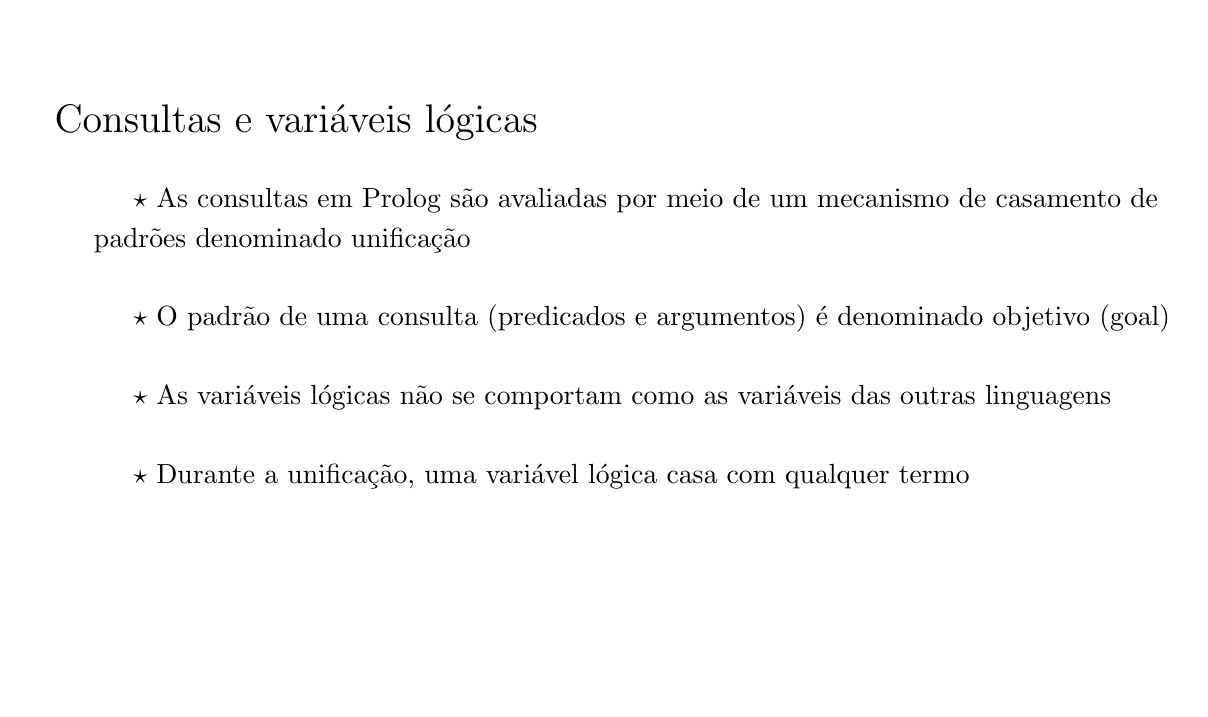
\begin{tikzpicture}
\node[draw,opacity=0] at (0, 0) {x};
\node[draw,opacity=0] at (14, 8) {x};

	\node[anchor=west] (title) at (0.0, 7.0) { \Large \bbbold{Consultas e variáveis lógicas} };


	\node[anchor=west] (a) at (1.0, 6.0) { $\star$ \bbtext{As consultas em Prolog são avaliadas por meio de um mecanismo de casamento de} };

	\node[anchor=west] (a1) at (0.5, 5.5) { \bbtext{padrões denominado \bbbold{unificação}} };


	\node[anchor=west] (b) at (1.0, 4.5) { $\star$ \bbtext{O padrão de uma consulta (predicados e argumentos) é denominado \bbbold{objetivo} (\bbenglish{goal})} };


	\node[anchor=west] (c) at (1.0, 3.5) { $\star$ \bbtext{As variáveis lógicas não se comportam como as variáveis das outras linguagens} };


	\node[anchor=west] (e) at (1.0, 2.5) { $\star$ \bbtext{Durante a unificação, uma variável lógica \bbbold{casa} com qualquer termo} };


\end{tikzpicture}
\end{frame}
\begin{frame}[plain,t]
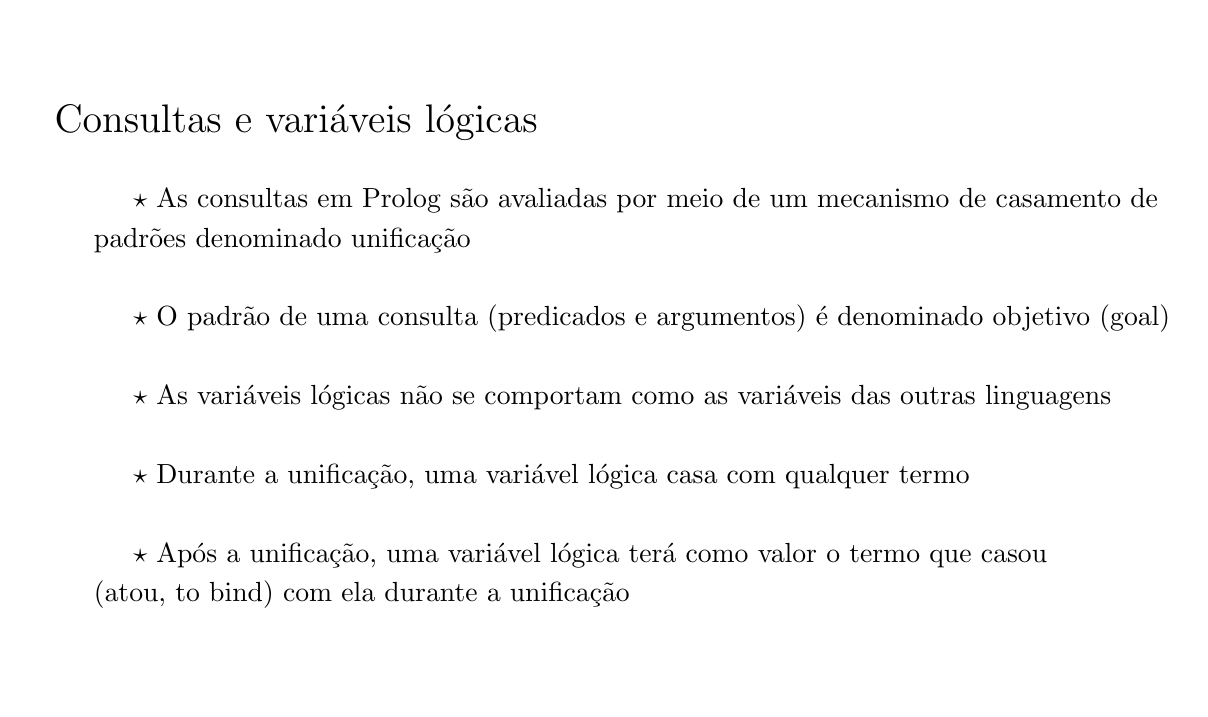
\begin{tikzpicture}
\node[draw,opacity=0] at (0, 0) {x};
\node[draw,opacity=0] at (14, 8) {x};

	\node[anchor=west] (title) at (0.0, 7.0) { \Large \bbbold{Consultas e variáveis lógicas} };


	\node[anchor=west] (a) at (1.0, 6.0) { $\star$ \bbtext{As consultas em Prolog são avaliadas por meio de um mecanismo de casamento de} };

	\node[anchor=west] (a1) at (0.5, 5.5) { \bbtext{padrões denominado \bbbold{unificação}} };


	\node[anchor=west] (b) at (1.0, 4.5) { $\star$ \bbtext{O padrão de uma consulta (predicados e argumentos) é denominado \bbbold{objetivo} (\bbenglish{goal})} };


	\node[anchor=west] (c) at (1.0, 3.5) { $\star$ \bbtext{As variáveis lógicas não se comportam como as variáveis das outras linguagens} };


	\node[anchor=west] (e) at (1.0, 2.5) { $\star$ \bbtext{Durante a unificação, uma variável lógica \bbbold{casa} com qualquer termo} };



	\node[anchor=west] (d) at (1.0, 1.5) { $\star$ \bbtext{Após a unificação, uma variável lógica terá como valor o termo que casou} };

	\node[anchor=west] (d1) at (0.5, 1.0) { \bbtext{(atou, \bbenglish{to bind}) com ela durante a unificação} };

\end{tikzpicture}
\end{frame}
\begin{frame}[plain,t]
\begin{tikzpicture}
\node[draw,opacity=0] at (0, 0) {x};
\node[draw,opacity=0] at (14, 8) {x};

	\node[anchor=west] (title) at (0.0, 7.0) { \Large \bbbold{Unificação} };

	\draw[fill=blue!10!white,rounded corners] (0.75, 6.0) rectangle  (13.5, 1.0);

	\draw[color=BBBlue,draw,very thick,rounded corners] (0.75, 6.0) rectangle  (13.5, 1.0);

	\draw[fill=BBBlue,color=BBBlue,draw,very thick,rounded corners] (0.75, 6.0) rectangle  (13.5, 5.0);


	\node[anchor=west,color=white] (a) at (1.0, 5.5) { \bbchalk{Versão simplificada} };

	\node[anchor=west,color=white] (b1) at (1.0, 4.5) { \bbtext{Se a base Prolog contém apenas fatos, a unificação é bem sucedida se as três} };

	\node[anchor=west,color=white] (b2) at (1.0, 3.75) { \bbtext{condições abaixo são satisfeitas:} };

	\node[anchor=west,color=white] (b3) at (1.5, 3.0) { \bbbold{1.} \bbtext{o predicado presente no objetivo e na base de dados é o mesmo} };

	\node[anchor=west,color=white] (b4) at (1.5, 2.25) { \bbbold{2.} \bbtext{ambos tem mesma aridade} };

	\node[anchor=west,color=white] (b5) at (1.5, 1.5) { \bbbold{3.} \bbtext{todos os argumentos são os mesmos} };

\end{tikzpicture}
\end{frame}
\begin{frame}[plain,t]
\vspace*{\fill}

\inputsnippet{prolog}{1}{19}{codes/unification.pl}

\vspace*{\fill}
\end{frame}
\begin{frame}[plain,t]
\vspace*{\fill}

\inputsnippet{prolog}{1}{19}{codes/variables.pl}

\vspace*{\fill}
\end{frame}
\begin{frame}[plain,t]
\vspace*{\fill}

\inputsnippet{prolog}{1}{19}{codes/same_var.pl}


\vspace*{\fill}
\end{frame}
\begin{frame}[plain,t]
\begin{tikzpicture}
\node[draw,opacity=0] at (0, 0) {x};
\node[draw,opacity=0] at (14, 8) {x};

	\node[anchor=west] (title) at (0.0, 7.0) { \Large \bbbold{Fatos dinâmicos} };

\end{tikzpicture}
\end{frame}
\begin{frame}[plain,t]
\begin{tikzpicture}
\node[draw,opacity=0] at (0, 0) {x};
\node[draw,opacity=0] at (14, 8) {x};

	\node[anchor=west] (title) at (0.0, 7.0) { \Large \bbbold{Fatos dinâmicos} };


	\node[anchor=west] (a) at (1.0, 6.0) { $\star$ \bbtext{Prolog permite a declaração ou retratação de fatos diretamente no interpretador} };

\end{tikzpicture}
\end{frame}
\begin{frame}[plain,t]
\begin{tikzpicture}
\node[draw,opacity=0] at (0, 0) {x};
\node[draw,opacity=0] at (14, 8) {x};

	\node[anchor=west] (title) at (0.0, 7.0) { \Large \bbbold{Fatos dinâmicos} };


	\node[anchor=west] (a) at (1.0, 6.0) { $\star$ \bbtext{Prolog permite a declaração ou retratação de fatos diretamente no interpretador} };


	\node[anchor=west] (b) at (1.0, 5.0) { $\star$ \bbtext{Para isto, o predicado deve ser declarado \bbbold{dinâmico}, por meio da diretiva \code{prolog}{dynamic}} };

\end{tikzpicture}
\end{frame}
\begin{frame}[plain,t]
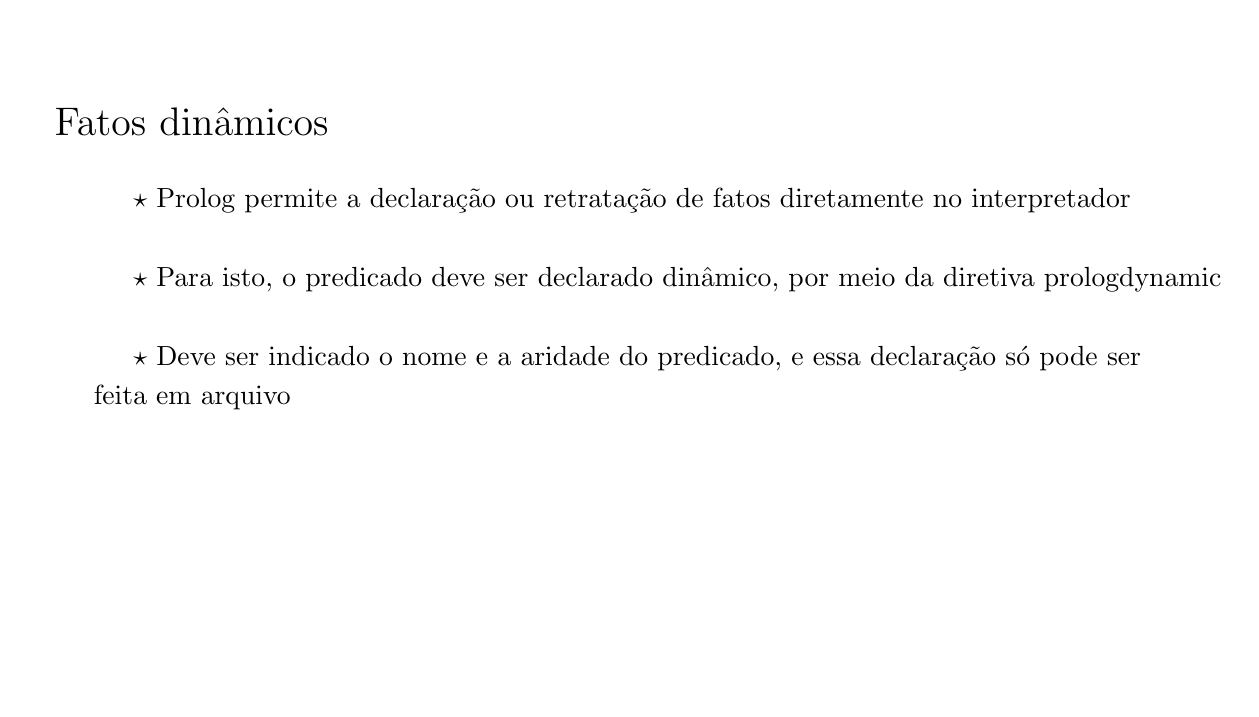
\begin{tikzpicture}
\node[draw,opacity=0] at (0, 0) {x};
\node[draw,opacity=0] at (14, 8) {x};

	\node[anchor=west] (title) at (0.0, 7.0) { \Large \bbbold{Fatos dinâmicos} };


	\node[anchor=west] (a) at (1.0, 6.0) { $\star$ \bbtext{Prolog permite a declaração ou retratação de fatos diretamente no interpretador} };


	\node[anchor=west] (b) at (1.0, 5.0) { $\star$ \bbtext{Para isto, o predicado deve ser declarado \bbbold{dinâmico}, por meio da diretiva \code{prolog}{dynamic}} };

	\node[anchor=west] (c) at (1.0, 4.0) { $\star$ \bbtext{Deve ser indicado o nome e a aridade do predicado, e essa declaração só pode ser} };

	\node[anchor=west] (c1) at (0.5, 3.5) { \bbtext{feita em arquivo} };

\end{tikzpicture}
\end{frame}
\begin{frame}[plain,t]
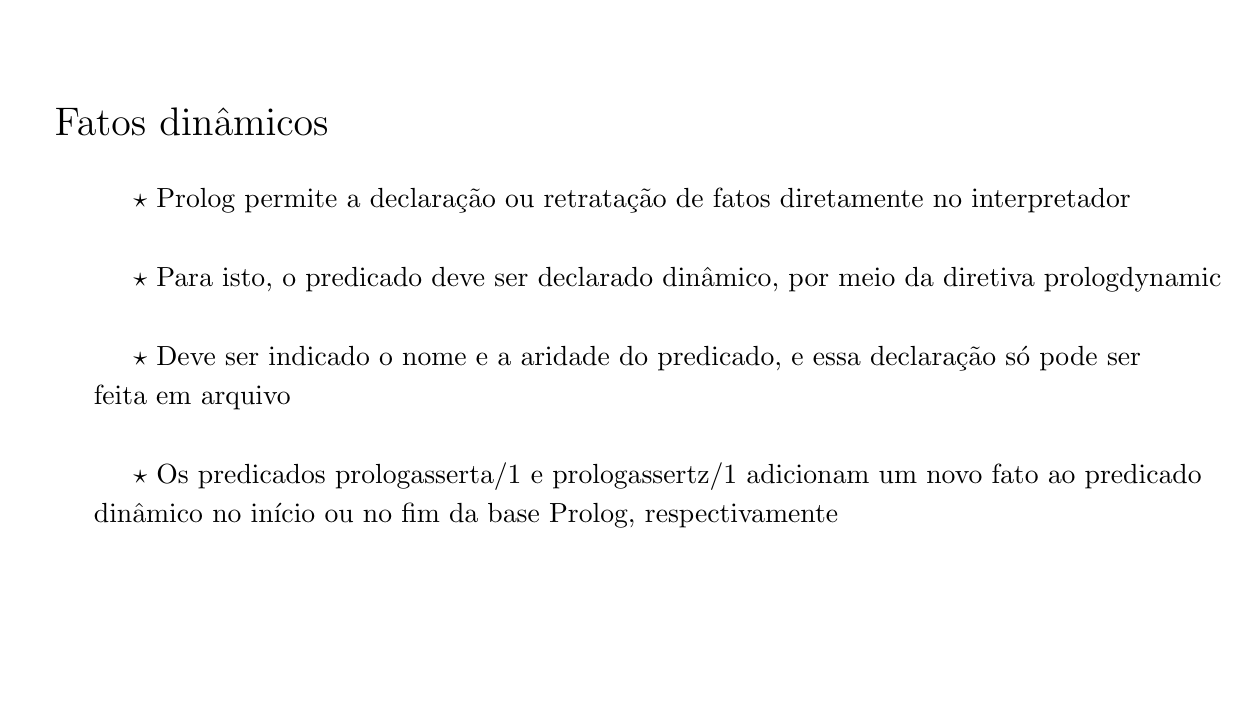
\begin{tikzpicture}
\node[draw,opacity=0] at (0, 0) {x};
\node[draw,opacity=0] at (14, 8) {x};

	\node[anchor=west] (title) at (0.0, 7.0) { \Large \bbbold{Fatos dinâmicos} };


	\node[anchor=west] (a) at (1.0, 6.0) { $\star$ \bbtext{Prolog permite a declaração ou retratação de fatos diretamente no interpretador} };


	\node[anchor=west] (b) at (1.0, 5.0) { $\star$ \bbtext{Para isto, o predicado deve ser declarado \bbbold{dinâmico}, por meio da diretiva \code{prolog}{dynamic}} };

	\node[anchor=west] (c) at (1.0, 4.0) { $\star$ \bbtext{Deve ser indicado o nome e a aridade do predicado, e essa declaração só pode ser} };

	\node[anchor=west] (c1) at (0.5, 3.5) { \bbtext{feita em arquivo} };

	\node[anchor=west] (d) at (1.0, 2.5) { $\star$ \bbtext{Os predicados \code{prolog}{asserta/1} e \code{prolog}{assertz/1} adicionam um novo fato ao predicado} };

	\node[anchor=west] (d1) at (0.5, 2.0) { \bbtext{dinâmico no início ou no fim da base Prolog, respectivamente} };

\end{tikzpicture}
\end{frame}
\begin{frame}[plain,t]
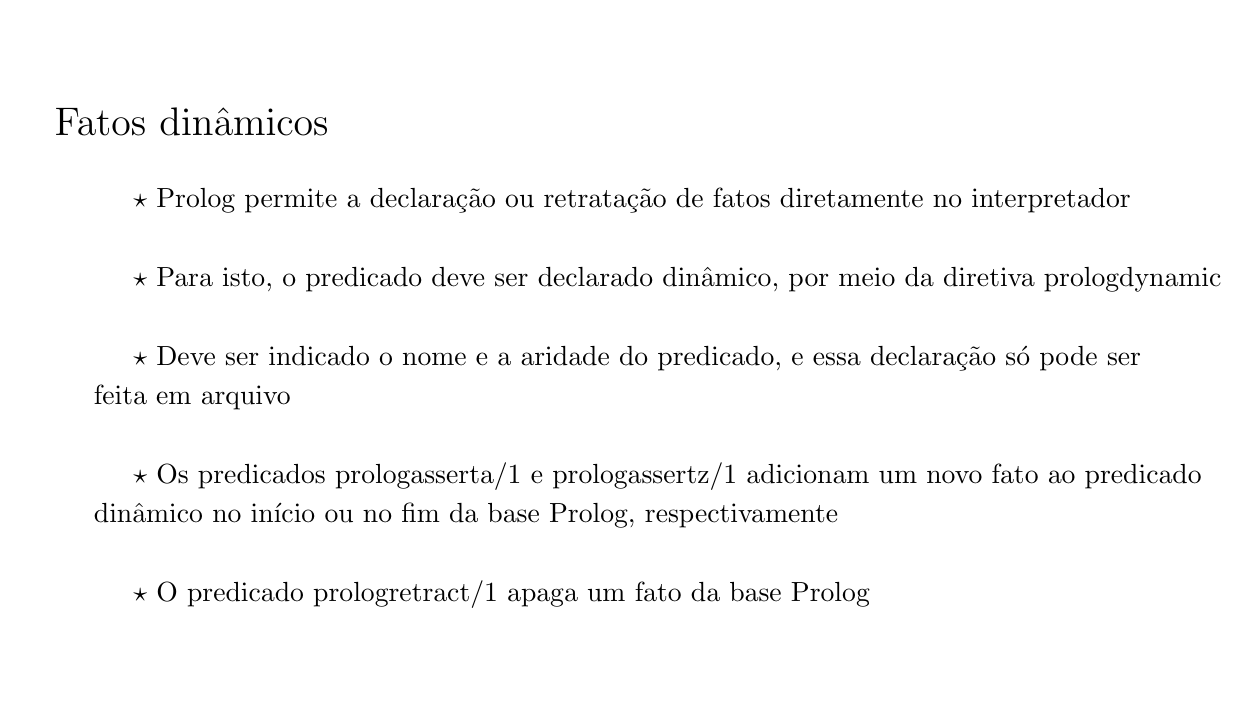
\begin{tikzpicture}
\node[draw,opacity=0] at (0, 0) {x};
\node[draw,opacity=0] at (14, 8) {x};

	\node[anchor=west] (title) at (0.0, 7.0) { \Large \bbbold{Fatos dinâmicos} };


	\node[anchor=west] (a) at (1.0, 6.0) { $\star$ \bbtext{Prolog permite a declaração ou retratação de fatos diretamente no interpretador} };


	\node[anchor=west] (b) at (1.0, 5.0) { $\star$ \bbtext{Para isto, o predicado deve ser declarado \bbbold{dinâmico}, por meio da diretiva \code{prolog}{dynamic}} };

	\node[anchor=west] (c) at (1.0, 4.0) { $\star$ \bbtext{Deve ser indicado o nome e a aridade do predicado, e essa declaração só pode ser} };

	\node[anchor=west] (c1) at (0.5, 3.5) { \bbtext{feita em arquivo} };

	\node[anchor=west] (d) at (1.0, 2.5) { $\star$ \bbtext{Os predicados \code{prolog}{asserta/1} e \code{prolog}{assertz/1} adicionam um novo fato ao predicado} };

	\node[anchor=west] (d1) at (0.5, 2.0) { \bbtext{dinâmico no início ou no fim da base Prolog, respectivamente} };

	\node[anchor=west] (e) at (1.0, 1.0) { $\star$ \bbtext{O predicado \code{prolog}{retract/1} apaga um fato da base Prolog} };

\end{tikzpicture}
\end{frame}
\begin{frame}[plain,t]
\vspace*{\fill}

\inputsnippet{prolog}{1}{20}{codes/dynamic.pl}

\vspace*{\fill}
\end{frame}
\begin{frame}[plain,t]
\vspace*{\fill}

\inputsnippet{prolog}{22}{42}{codes/dynamic.pl}

\vspace*{\fill}
\end{frame}
\begin{frame}[plain,t]
\begin{tikzpicture}
\node[draw,opacity=0] at (0, 0) {x};
\node[draw,opacity=0] at (14, 8) {x};

	\node[anchor=west] (title) at (0.0, 7.0) { \Large \bbbold{Quantificador universal} };

	\draw[fill=blue!10!white,rounded corners] (0.75, 5.5) rectangle  (13.5, 2.0);

	\draw[color=BBBlue,draw,very thick,rounded corners] (0.75, 5.5) rectangle  (13.5, 2.0);

	\draw[fill=BBBlue,color=BBBlue,draw,very thick,rounded corners] (0.75, 5.5) rectangle  (13.5, 4.5);


	\node[anchor=west,color=white] (a) at (1.0, 5.0) { \bbchalk{Definição} };

	\node[anchor=west,color=white] (b1) at (1.0, 4.0) { \bbtext{Sejam $S(x)$ uma sentença aberta. O quantificador \bbbold{universal} $\forall$ é utilizado na} };

	\node[anchor=west,color=white] (b2) at (1.0, 3.25) { \bbtext{construção $\forall x.S(x)$, a qual significa que, para todos os valores $v$ no conjunto} };

	\node[anchor=west,color=white] (b3) at (1.0, 2.5) { \bbtext{universal de $x$, $S(v)$ é verdadeira.} };

\end{tikzpicture}
\end{frame}
\begin{frame}[plain,t]
\begin{tikzpicture}
\node[draw,opacity=0] at (0, 0) {x};
\node[draw,opacity=0] at (14, 8) {x};

	\node[anchor=west] (title) at (0.0, 7.0) { \Large \bbbold{Generalizações} };

\end{tikzpicture}
\end{frame}
\begin{frame}[plain,t]
\begin{tikzpicture}
\node[draw,opacity=0] at (0, 0) {x};
\node[draw,opacity=0] at (14, 8) {x};

	\node[anchor=west] (title) at (0.0, 7.0) { \Large \bbbold{Generalizações} };


	\node[anchor=west] (a) at (1.0, 6.0) { $\star$ \bbtext{O quantificador universal é expresso, em Prolog, por meio de uma \bbbold{generalização}} };

\end{tikzpicture}
\end{frame}
\begin{frame}[plain,t]
\begin{tikzpicture}
\node[draw,opacity=0] at (0, 0) {x};
\node[draw,opacity=0] at (14, 8) {x};

	\node[anchor=west] (title) at (0.0, 7.0) { \Large \bbbold{Generalizações} };


	\node[anchor=west] (a) at (1.0, 6.0) { $\star$ \bbtext{O quantificador universal é expresso, em Prolog, por meio de uma \bbbold{generalização}} };


	\node[anchor=west] (b) at (1.0, 5.0) { $\star$ \bbtext{Generalizações são fatos que casam com qualquer valor} };

\end{tikzpicture}
\end{frame}
\begin{frame}[plain,t]
\begin{tikzpicture}
\node[draw,opacity=0] at (0, 0) {x};
\node[draw,opacity=0] at (14, 8) {x};

	\node[anchor=west] (title) at (0.0, 7.0) { \Large \bbbold{Generalizações} };


	\node[anchor=west] (a) at (1.0, 6.0) { $\star$ \bbtext{O quantificador universal é expresso, em Prolog, por meio de uma \bbbold{generalização}} };


	\node[anchor=west] (b) at (1.0, 5.0) { $\star$ \bbtext{Generalizações são fatos que casam com qualquer valor} };


	\node[anchor=west] (c) at (1.0, 4.0) { $\star$ \bbtext{Por exemplo, considere o predicado \code{prolog}{is_term/1}, definido abaixo:} };

	\node[anchor=west] (c1) at (2.0, 3.0) { \code{prolog}{is_term(X).} };

\end{tikzpicture}
\end{frame}
\begin{frame}[plain,t]
\begin{tikzpicture}
\node[draw,opacity=0] at (0, 0) {x};
\node[draw,opacity=0] at (14, 8) {x};

	\node[anchor=west] (title) at (0.0, 7.0) { \Large \bbbold{Generalizações} };


	\node[anchor=west] (a) at (1.0, 6.0) { $\star$ \bbtext{O quantificador universal é expresso, em Prolog, por meio de uma \bbbold{generalização}} };


	\node[anchor=west] (b) at (1.0, 5.0) { $\star$ \bbtext{Generalizações são fatos que casam com qualquer valor} };


	\node[anchor=west] (c) at (1.0, 4.0) { $\star$ \bbtext{Por exemplo, considere o predicado \code{prolog}{is_term/1}, definido abaixo:} };

	\node[anchor=west] (c1) at (2.0, 3.0) { \code{prolog}{is_term(X).} };


	\node[anchor=west] (d) at (1.0, 2.0) { $\star$ \bbtext{Ele é verdadeiro para qualquer argumento \code{prolog}{X}: de fato, o argumento de um predicado} };

	\node[anchor=west] (d1) at (0.5, 1.5) { \bbtext{deve ser um termo, de modo que a implementação está semanticamente correta} };

\end{tikzpicture}
\end{frame}
\begin{frame}[plain,t]
\begin{tikzpicture}
\node[draw,opacity=0] at (0, 0) {x};
\node[draw,opacity=0] at (14, 8) {x};

	\node[anchor=west] (title) at (0.0, 7.0) { \Large \bbbold{Generalizações} };


	\node[anchor=west] (a) at (1.0, 6.0) { $\star$ \bbtext{O quantificador universal é expresso, em Prolog, por meio de uma \bbbold{generalização}} };


	\node[anchor=west] (b) at (1.0, 5.0) { $\star$ \bbtext{Generalizações são fatos que casam com qualquer valor} };


	\node[anchor=west] (c) at (1.0, 4.0) { $\star$ \bbtext{Por exemplo, considere o predicado \code{prolog}{is_term/1}, definido abaixo:} };

	\node[anchor=west] (c1) at (2.0, 3.0) { \code{prolog}{is_term(X).} };


	\node[anchor=west] (d) at (1.0, 2.0) { $\star$ \bbtext{Ele é verdadeiro para qualquer argumento \code{prolog}{X}: de fato, o argumento de um predicado} };

	\node[anchor=west] (d1) at (0.5, 1.5) { \bbtext{deve ser um termo, de modo que a implementação está semanticamente correta} };


	\node[anchor=west] (e) at (1.0, 0.5) { $\star$ \bbtext{Uma vez que a variável \code{prolog}{X} não é utilizada no corpo da regra, ela pode ser} };

	\node[anchor=west] (e1) at (0.5, 0.0) { \bbtext{substituída pelo \bbenglish{wildcard} `\code{prolog}{_}'} };


\end{tikzpicture}
\end{frame}
\begin{frame}[plain,t]
\vspace*{\fill}

\inputsnippet{prolog}{1}{17}{codes/is_term.pl}

\vspace*{\fill}
\end{frame}
\begin{frame}[plain,t]
\begin{tikzpicture}
\node[draw,opacity=0] at (0, 0) {x};
\node[draw,opacity=0] at (14, 8) {x};

	\node[anchor=west] (title) at (0.0, 6.5) { \Large \bbbold{Referências} };

	\node[anchor=west] (a) at (1.0, 2.0) { $\star$ \bbbold{SWI-Prolog.} \bbenglish{https://www.swi-prolog.org/,} \bbtext{acesso em 10/03/2026.} };

	\node[anchor=west] (b) at (1.0, 4.0) { $\star$ \bbbold{LibreTexts Mathematics.} \bbenglish{Open Sentences and Sets,} \bbtext{acesso em 10/03/2026.} };

	\node[anchor=west] (c) at (1.0, 1.0) { $\star$ \bbbold{Wikipédia.} \bbenglish{Prolog syntax and semantics,} \bbtext{acesso em 10/03/2026.} };

	\node[anchor=west] (d) at (1.0, 3.0) { $\star$ \bbbold{MERRIT}\bbtext{, Dennis.} \bbenglish{Adventure in Prolog, Amzi!,} \bbtext{191 pgs, 2017.} };

	\node[anchor=west] (e) at (1.0, 5.0) { $\star$ \bbbold{Banco Central do Brasil.} \bbenglish{Cotações e boletins,} \bbtext{acesso em 10/03/2026.} };

\end{tikzpicture}
\end{frame}
\end{document}
